\section{Categorical Normalizing Flows}
\label{sec:methodology}

The review of related work has shown that while normalizing flows on categorical distribution exist, they are limited in their expressiveness due to discretizing the change of variable formula.
Continuous normalizing flows, on the other hand, are significantly more powerful.
Motivated by these limitations, we present Categorical Normalizing Flows that jointly learn an encoding distribution to continuous space for categorical data and a consecutive normalizing flow on this continuous representation.
We discuss the details of this approach in Section~\ref{sec:methodology_CNF}.
In the second part, Section~\ref{sec:methodology_GraphCNF}, we introduce GraphCNF, a Categorical Normalizing Flow on graph modeling which is permutation-invariant to the node order. 

\subsection{Continuous Normalizing Flows on Categorical Data}
\label{sec:methodology_CNF}

We define $\bm{x}$ to be a multivariate, nominal discrete random variable, where each element $x_i$ is a categorical variable of $K$ categories with no intrinsic order.
Our goal is to learn the joint probability mass function, $P_{\text{model}}(\bm{x})$, via a normalizing flow.
As normalizing flows originally constitute a class of continuous transformations, it is not directly possible to rely on them for modeling $P_{\text{model}}(\bm{x})$. Instead, we propose to learn a continuous latent space 
in which each categorical choice of a variable $x_i$ maps to one distribution of a continuous variable $\bm{z}_i \in \mathbb{R}^{d}$. 
Thereby, we want to have the following properties:
\begin{itemize}
	\item The continuous distributions corresponding to different categories should be non-overlapping to preserve unique decoding, similar to current dequantization methods. Specifically, the latent space is ideally partitioned into $K$ regions, one for each category. This ensures that no information is lost when mapping the discrete data to continuous values.
	\item In contrast to integers, categories do not have an intrinsic order which would provide a natural positioning of the non-overlapping volumes.
	However, there usually exist (hidden) relations between the categories which are beneficial to represent in the encoding.
	Thus, the positioning of the volumes and distributions per category need to be jointly optimized with the continuous flow $p_{\text{model}}(\bm{z})$ instead of pre-specified.
	\item Relations between data points are usually represented by distance in continuous space. Categories can have several multi-dimensional relations as it is the case for words and their meaning. To encode those relations into the latent space, a single dimension is not sufficient as it cannot represent all the different forms of relations. Thus, the encoding distribution needs to support an arbitrary number of dimensions for $\bm{z}_i$.
\end{itemize}
In summary, the optimal encoding distribution would learn a partitioning of the continuous latent space into $K$ volumes, each representing one category with a flexible distribution within this part.

\subsubsection{Encoding categorical data into continuous latent space}

In order to find such a function, we propose to learn a flexible encoding distribution $q(\bm{z}|\bm{x})$ by simultaneously optimizing a decoder $p(\bm{x}|\bm{z})$ for the reverse mapping. 
This allows us to jointly optimize the encoding of the categorical data with the normalizing flow on the continuous representation. 
A common framework for learning such an encoder-decoder structure on distributions is variational inference \cite{VAE, NormalizingFlowsFundamentals}. 
However, variational inference in the form as presented above has two drawbacks. 
Firstly, defining a joint decoder distribution does not fulfill our desired property of partitioning the latent space. 
Instead, the encoder-decoder model will compress the information as the decoder can infer categories from other continuous variables, which also leads to overlaps in distributions per category. 
However, we want the interaction of the variables to be learned in the normalizing flow to utilize its parallel sampling and exact density evaluation.
Secondly, $p(\bm{x}|\bm{z})$ represents an approximate posterior of the likelihood $q(\bm{z}|\bm{x})$. The difference between the true and approximate posterior is the KL-divergence $D_{KL}(p(\bm{x}|\bm{z})||q(\bm{x}|\bm{z}))$, which cannot be determined as $q(\bm{x}|\bm{z})$ is unknown.
Thus, we can only model a lower bound which tends to increasingly diverge with the true posteriors' complexity \cite{VAEDeeperUnderstanding, VAEAdvances}. 

To overcome these issues, we propose to simplify the decoder by factorizing the posterior: $p(\bm{x}|\bm{z})=\prod_i p(x_i|\bm{z}_i)$. 
This limits the variational inference framework to a toolkit for learning the optimal partitioning of the latent space. 
Factorizing the posterior distribution means that we assume independence between the categorical variables given their learned continuous encodings. 
Therefore, any interaction between the categorical variables $\bm{x}$ must be learned inside the normalizing flow.
On the other hand, the encoder $q(\bm{z}|\bm{x})$ is being optimized to provide suitable representations of the categorical variables to the flow while separating the different categories in latent space to improve the decoding. The KL divergence between true and approximate posterior is also expected to be close to zero as the posterior becomes almost deterministic. 
Overall, our objective becomes:
\begin{equation}
	\E_{\bm{x}\sim P_{\text{data}}}\left[\log P_{\text{model}}(\bm{x})\right] \geq \E_{\bm{x}\sim P_{\text{data}}}\E_{\bm{z}\sim q(\cdot|\bm{x})}\left[\log \frac{p_{\text{model}}(\bm{z}) \prod_i p(x_i|\bm{z}_i)}{q(\bm{z}|\bm{x})}\right]
\end{equation}
We refer to this framework as \emph{Categorical Normalizing Flows}. In contrast to dequantization in Equation~\ref{eqn:related_work_dequantization_variational}, the continuous encoding $\bm{z}$ is not bounded by the domain of the encoding distribution. 
Instead, the partitioning is jointly learned with the model likelihood. 
Furthermore, we can freely choose the dimensionality of the continuous variables, $\bm{z}_i$, to fit the number of categories and their relations. 
This can be crucial for large sets of categories or distributions with complex interactions among categorical variables, as we show in experiments on graph coloring and language modeling (see Section~\ref{sec:experiments_graph_coloring} and \ref{sec:experiments_language_modeling}).

\subsubsection{Flexibility of encoder distribution}

In the variational inference framework, the encoder $q(\bm{z}|\bm{x})$ and decoder $p(x_i|\bm{z}_i)$ can be implemented in several ways. 
To this extent, we consider three possible encoding distributions with increasing complexity: a mixture model, linear flows, and variational encoding. 
We compare the encoding distribution in experiments in Section~\ref{sec:experiments_set_modeling}, and detail them in the following paragraphs.

\paragraph{Mixture model} The mixture model represents each category by an independent logistic distribution in continuous latent space, as visualized in Figure~\ref{fig:methodology_encoding_dist_mixt}.
Specifically, the encoder distribution $q(\bm{z}|\bm{x})$, with $\bm{x}$ being the categorical input and $\bm{z}$ the continuous latent representation, can be written as:
\begin{eqnarray}
    q(\bm{z}|\bm{x}) & = & \prod_{i=1}^{N} g(\bm{z}_i|\mu(x_i), \sigma(x_i))\\
    g(\bm{v}|\mu, \sigma) & = & \prod_{j=1}^{d} \frac{\exp(-\epsilon_j)}{\left(1+\exp(-\epsilon_j)\right)^2}\hspace{2mm}\text{where}\hspace{2mm}\epsilon_j=\frac{v_j-\mu_j}{\sigma_j}
\end{eqnarray}
$g$ represent the logistic distribution, and $d$ the dimensionality of the continuous latent space per category. Both parameters $\bm{\mu}\in\mathbb{R}^{d}$ and $\sigma\in\mathbb{R}_{>0}^{d}$ are learnable parameter, which can be implemented via a simple table lookup. 
In this setup, the true posterior can actually be found and efficiently calculated by applying the Bayes rule:
\begin{equation}
    p(x_i|\bm{z}_i) = \frac{\tilde{p}(x_i)q(\bm{z}_i|x_i)}{\sum_{\hat{x}}\tilde{p}(\hat{x})q(\bm{z}_i|\hat{x})}
\end{equation}
where the prior over categories, $\tilde{p}(x_i)$, is calculated based on the category frequencies in the training dataset. 
Finding the true posterior ensures that no additional lower bound is added to the likelihood objective by the variational inference framework.
Furthermore, the distribution is strongly peaked for most continuous points in the latent space as the model is trained to minimize the posterior entropy which pushes the posterior to be deterministic for frequently sampled continuous points. 
Hence, the posterior partitions the latent space into fragments in which all continuous points are assigned to one discrete category. 
The gaps between the fragments, where the posterior is not close to deterministic, are small and very rarely sampled by the encoder distribution. 
A visualization of the partitioning for an example of three categories is shown in Figure~\ref{fig:methodology_encoding_dist_mixt}. 

\begin{figure}[t!]
    \centering
    \setlength{\tabcolsep}{20pt}
    \begin{tabular}{cc}
        \includegraphics[width=0.28\textwidth]{figures/appendix_figures/encoding_dist_mixture_pure.pdf} & \includegraphics[width=0.28\textwidth]{figures/appendix_figures/encoding_dist_mixture.pdf} \\[3.5mm]
        (a) Encoding distribution $q(\bm{z}_i|x_i)$ & (b) Posterior partitioning $p(x_i|\bm{z_i})$ \\
    \end{tabular}
    \caption[Mixture model encoding]{Visualization of the mixture model encoding and decoding for 3 categories. Best viewed in color. (a) Each category is represented by a logistic distribution with independent mean and scale which are learned during training. (b) The posterior partitions the latent space which is visualized by the background color. The borders show from when on we have an almost unique decoding of the corresponding mixture ($>0.95$ decoding probability). Note that these borders do not directly correspond to the euclidean distance as we use logistic distributions instead of Gaussians.}
    \label{fig:methodology_encoding_dist_mixt}
\end{figure}

Besides a logistic distribution, any other continuous distributions with support over $\mathbb{R}^{d}$ such as Gaussian can also be used for $g(\bm{z}_i)$.
Still, our selection of taking a logistic is based on suitable designs of the continuous normalizing flow $p_{\text{model}}(\bm{z})$, in particular the logistic mixture coupling layer \cite{Flow++} (see Section~\ref{sec:background_comparing_coupling_layers} for a review on this flow layer). 
The logistic mixture layer maps $K$ logistics back into a single mode.
This is particularly useful in Categorical Normalizing Flows if the encoding distribution is a mixture of logistics as the goal of the continuous flow is to map this mixture back to the base distribution which again is a logistic distribution.
Furthermore, it can be shown that for a one-layer autoregressive flow with as many mixtures as the number of categories in the discrete distribution, the likelihood objective falls back to the one of a standard recurrent neural network. 
The proof is detailed in Appendix~\ref{sec:appendix_mixture_optimality}.
This statement implies that an autoregressive Categorical Normalizing Flow can be at least as powerful as an RNN with the same neural network, which has not been the case in previous work \cite{SemiDiscreteNFSequence}.  
Also for non-autoregressive flows, logistic mixture layers provide a strong framework as fewer transformations are needed to accurately model the continuous input distribution. 

\paragraph{Linear flows} Representing each category by a simple logistic distribution considerably limits the encoder's flexibility. 
This flexibility can be increased by applying normalizing flows on each mixture that dependent on the discrete category. 
We refer to this approach as \textit{linear flows} as the flows are applied for each categorical input variable independently.
Formally, we can write the distribution as: 
\begin{eqnarray}
    q(\bm{z}|\bm{x}) & = & \prod_{i=1}^{N} q(\bm{z}_i|x_i)\\
    q\left(\bm{z}^{(K)}\big\vert x_i\right) & = & g\left(\bm{z}^{(0)}\right) \cdot \prod_{k=1}^{K} \left|\det \frac{\partial f_k(\bm{z}^{(k-1)}; x_i)}{\partial \bm{z}^{(k-1)}}\right|\hspace{2mm}\text{where}\hspace{2mm}\bm{z}_i=\bm{z}^{(K)}
\end{eqnarray}
where $f_1,...,f_K$ are invertible, smooth transformations and $g$ represents a logistic distribution with $\mu=0, \sigma=1$. 
In particular, we use here a sequence of coupling layers with activation normalization and invertible 1x1 convolutions \cite{Glow}. 
Both the activation normalization and coupling use the category $x_i$ as an additional external input to determine their transformation parameters by a neural network. 
The class-conditional transformations could also be implemented by storing $K$ parameter sets for the coupling layer neural networks, which is however inefficient for a larger number of categories.  
An example of possible encoding distributions with linear flows is visualized in Figure~\ref{fig:methodology_encoding_dist_linear_flows}. 

\begin{figure}[t!]
    \centering
    \setlength{\tabcolsep}{20pt}
    \begin{tabular}{cc}
        \includegraphics[width=0.28\textwidth]{figures/appendix_figures/encoding_dist_linear_flows_pure.pdf} & \includegraphics[width=0.28\textwidth]{figures/appendix_figures/encoding_dist_linear_flows.pdf} \\[3.5mm]
        (a) Encoding distribution $q(\bm{z}_i|x_i)$ & (b) Posterior partitioning $p(x_i|\bm{z_i})$ \\
    \end{tabular}
    \caption[Linear flow encoding]{Visualization of the linear flow encoding and decoding for 3 categories. Best viewed in color. (a) The distribution per category is not restricted to a simple logistic and can be multi-modal, rotated or transformed even more. (b) The posterior partitions the latent space which is visualized by the background color. The borders show from when on we have an almost unique decoding of the corresponding category distribution ($>0.95$ decoding probability). Those borders can take any form due to the posteriors flexibility.}
    \label{fig:methodology_encoding_dist_linear_flows}
\end{figure}

Similarly to the mixture model, we can calculate the true posterior $p(x_i|\bm{z}_i)$ using Bayes rule. 
Thereby, we sample from the flow for $x_i$ and need to invert the flows for all other categories. 
Note that as the inverse of the flow also needs to be differentiable by stochastic gradient descend in this situation, we apply affine coupling layers instead of logistic mixture layers.
However, executing linear flows for every categorical variable becomes computationally expensive when there exist more than 20 categories, and thus we use a single-layer linear network as posterior in these cases.


\paragraph{Variational encoding}
The third encoding distribution we experimented with is inspired by variational dequantization \cite{Flow++} and models $q(\bm{z}|\bm{x})$ by one flow across all categorical variables.
With this setup, the encoder distribution can model dependencies across categorical variables and allows even more complex representations than linear flows.
Nevertheless, the posterior, $p(x_i|\bm{z}_i)$, is still applied for each categorical variable independently to maintain the unique decoding and partitioning of the latent space. 
Thus, although the distribution for a category depends on the entire input $\bm{x}$ and the continuous representation of the other variables, all representations of this category are limited to their part in the latent space.
For instance, the category $a$ in the input $\bm{x}=[a,b]$ can be differently represented than in the input $\bm{x}=[a,c]$, but both distribution lie in the same partition modeled by the posterior. 
As the true posterior cannot be found for this distribution, we apply a small linear network to determine $p(x_i|\bm{z}_i)$. 


\subsection{Graph generation with Categorical Normalizing Flows}
\label{sec:methodology_GraphCNF}
Categorical Normalizing Flows can be applied to any task involving categorical data, of which one is graph modeling.
A graph $\mathcal{G}=(V,E)$ is defined by a set of nodes $V$ and a set of edges $E$ whose elements can have attributes that are often categorical. 
When modeling a graph, both the attributes and the overall graph structure need to be considered.
The most successful current approaches \cite{GraphRNNAttention, MolecularRNN, GraphAF, GraphRNN} are autoregressive although graphs are usually not sequential data. \citet{OrderMatters} has shown that treating set-like data as a sequence can significantly hurt performance, and we validate this issue in experiments on graph coloring in Section~\ref{sec:experiments_graph_coloring}. 
Furthermore, a likelihood-based model should intuitively assign equal probability to any permutation or order of the nodes as all of them represent the same graph.

Starting from Categorical Normalizing Flows, we propose GraphCNF, a normalizing flow for graph generation that is invariant to the order of nodes by generating all nodes and edges at once.
Given a graph $\mathcal{G}$, we model each node and edge as a separate categorical variable where the categories correspond to their discrete attributes. 
However, we also need to model whether there exists an edge between two nodes at all or not, as this changes across graphs. 
We implement this by adding an extra category to the edges representing the missing or \textit{virtual} edges. 
Hence, to model an arbitrary graph, we consider an edge variable for every possible tuple of nodes.
To apply normalizing flows on the node and edge categorical variables, we map them into continuous latent space using Categorical Normalizing Flows. 
Subsequent coupling layers map those representations to a continuous prior distribution.
Thereby, GraphCNF uses two crucial design choices for graph modeling: (1) we perform the generation stepwise for improved efficiency, and (2) we ensure that the model assigns an equal likelihood to any ordering of the nodes.

\begin{figure}[t!]
	\centering
	\includegraphics[width=\textwidth]{figures/methodology_figures/GraphCNF.pdf}
	\caption[Model architecture of GraphCNF]{Visualization of GraphCNF for an example graph of five nodes. We add the node and edge attributes, as well as the virtual edges stepwise to the latent space while leveraging the graph structure in the coupling layers. The last step considers a fully connected graph with features per edge.
	}
	\label{fig:methodology_graph_flow}
\end{figure}

\subsubsection{Three-step generation}
Modeling all edges including the virtual ones requires a significant amount of latent variables and is computationally expensive.
However, normalizing flows have been shown to benefit from splitting of latent variables at earlier layers while increasing efficiency \cite{RealNVP, Glow}. 
Furthermore, generating nodes based on the graph structure is a significantly easier task than jointly modeling the nodes with the edges as previous work has shown \cite{GraphNVP}.
Thus, we propose to add the node types, edge attributes, and graph structure stepwise to the latent space as visualized in Figure~\ref{fig:methodology_graph_flow}. 

In the first step, we encode the nodes into continuous latent space, $\bm{z}_0^{(V)}$, using Categorical Normalizing Flows. On those, we apply a group of coupling layers, $f_1$, which additionally use the adjacency matrix and the edge attributes, denoted by $E_{attr}$, as input. Thus, we can summarize the first step as:
\begin{eqnarray}
    z_{1}^{(V)} & = & f_1\big(z_{0}^{(V)}; E, E_{attr}\big)
\end{eqnarray}
The second step incorporates the edge attributes, $E_{attr}$, into latent space. Hence, all edges of the graph except the virtual edges are encoded into latent variables, $\bm{z}_0^{(E_{attr})}$, representing their attribute. The following coupling layers, denoted by $f_2$, transform both the node and edge attribute variables:
\begin{eqnarray}
    z_{2}^{(V)}, z_{1}^{(E_{attr})} & = & f_2\big(z_{1}^{(V)}, z_{0}^{(E_{attr})}; E\big)
\end{eqnarray}
Finally, we add the virtual edges to the latent variable model as $z_{0}^{(E^*)}$. Thereby, we need to slightly adjust our encoding from Categorical Normalizing Flows as we considered the virtual edges as an additional category of the edges. 
While the other categories are already encoded by $\bm{z}_{1}^{(E_{attr})}$, we add a separate encoding distribution for the virtual edges.
This distribution is modeled by a logistic base distribution with one additional flow layer (affine coupling, activation normalization, and invertible 1x1 convolution).
Meanwhile, the decoder needs to be applied on all edges, as we have to distinguish the continuous representation between virtual and non-virtual edges. 
Overall, the mapping can be summarized as:
\begin{eqnarray}
    z_{3}^{(V)}, z_{1}^{(E)} & = & f_3\big(z_{2}^{(V)}, z_{0}^{(E)}\big)\hspace{3mm}\text{where}\hspace{3mm}z_{0}^{(E)} = \big[z_{1}^{(E_{attr})}, z_{0}^{(E^*)}\big]
\end{eqnarray}
where the latent variables $z_{3}^{(V)}$ and $z_{1}^{(E)}$ are trained to follow a prior distribution. 
During sampling, we first invert $f_3$ and determine the general graph structure. Next, we invert $f_2$ and reconstruct the edge attributes. Finally, we apply the inverse of $f_1$ and determine the node types. 

\subsubsection{Permutation-invariant graph modeling}
To make sure that the transformations of the coupling layers are permutation invariant,
we apply a channel masking strategy \cite{RealNVP} such that the split between latent variables is independent of the order of the nodes.
Specifically, the split is performed over the latent dimensions for each node and edge independently.
Secondly, we leverage the graph structure in the coupling networks by applying graph neural networks. 
In the first step, $f_1$, we use a Relation GCN \cite{RGCN} which incorporates the categorical edge attributes into the layer.
For the second and third step, we need a graph network that supports the modeling of both node and edge features.
We refer to this network as Edge-GNN, and we found that various implementations work well.
The specific layer we used is described in the next paragraph.
Using both design choices, GraphCNF assigns equal probability to any ordering of nodes in a graph.

\paragraph{Edge-GNN} GraphCNF implements a three-step generation approach, for which the second and third step also models latent variables for edges. Hence, in the coupling layers, we need a graph neural network which supports both node and edge features. We implement this by alternating between updates of the edge and the node features. Specifically, given node features $\bm{v}^{t}$ and edge features $\bm{e}^{t}$ at layer $t$, we update those as follows:
\begin{eqnarray}
    \bm{v}^{t+1} & = & f_{node}(\bm{v}^{t}; \bm{e}^{t})\\
    \bm{e}^{t+1} & = & f_{edge}(\bm{e}^{t}; \bm{v}^{t+1})
\end{eqnarray}
The update functions, $f_{node}$ and $f_{edge}$, are both common graph neural network layers with slight adjustments to allow a communication between nodes and edges. 
Before detailing the update layers, it should be noted that we use Highway GNNs \cite{HighwayGNN} which apply a gating mechanism. 
Specifically, the updates for the nodes are determined by:
\begin{eqnarray}
    \bm{v}^{t+1} & = & \bm{v}^{t} \cdot T\left(\tilde{\bm{v}}^{t+1}\right) + H\left(\tilde{\bm{v}}^{t+1}\right) \cdot \left(1 - T\left(\tilde{\bm{v}}^{t+1}\right)\right)
\end{eqnarray}
where $\tilde{\bm{v}}^{t+1}$ is the output of the GNN layer. 
$H$ and $T$ represent single linear layer networks where $T$ has a consecutive sigmoid activation to limit the outputs between 0 and 1. 
The edge updates are applied similarly. 
We experienced that such a gated update function helps the gradient flow through the layers back to the input. 
This is important for normalizing flows as coupling layers or transformations in general strongly depend on previous transformations. 
Hence, we apply the same gating mechanism in the first step of GraphCNF, $f_1$.

\begin{figure}[t!]
    \centering
    \begin{subfigure}{.3\textwidth}
        \centering
        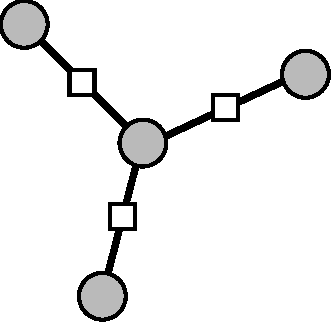
\includegraphics[height=3.5cm]{figures/methodology_figures/EdgeGNN/example_graph.pdf}
        \caption{Example graph}
        \label{fig:methodology_edgeGNN_example_graph}
    \end{subfigure}
    \hfill
    \begin{subfigure}{.3\textwidth}
        \centering
        \vfill
        \includegraphics[height=3.5cm]{figures/methodology_figures/EdgeGNN/edge_update.pdf}
        \caption{Edge update $f_{edge}$}
        \label{fig:methodology_edgeGNN_edge_update}
    \end{subfigure}
    \hfill
    \begin{subfigure}{.3\textwidth}
        \centering
        \includegraphics[height=3.5cm]{figures/methodology_figures/EdgeGNN/node_update.pdf}
        \caption{Node update $f_{node}$}
        \label{fig:methodology_edgeGNN_node_update}
    \end{subfigure}
    \caption[Edge and node udpates in EdgeGNN]{
    High-level visualization of the feature updates in EdgeGNN on an example graph (a). (b) The edge features are updated by taking into account the adjacent nodes. (c) For the node features, both the features of the neighbouring nodes as well as its edges are taken into consideration. For readability, only the update of the center node is shown although the features of all nodes are updated in parallel.}
    \label{fig:methodology_edgeGNN}
\end{figure}

Next, we detail the GNN layers to obtain $\tilde{\bm{e}}^{t+1}$ and $\tilde{\bm{v}}^{t+1}$. 
A visualization of the interaction between edge and node features in the updates is shown in Figure~\ref{fig:methodology_edgeGNN}.
The edge update layer $f_{edge}$ resembles a graph convolutional layer \cite{GraphOverview1}, and can be specified as follows:
\begin{equation}
	\tilde{e}^{t+1}_{ij} = g\left({W}^{t}_e e^{t}_{ij} + {W}^{t}_v v^{t}_{i} + {W}^{t}_v v^{t}_{j}\right)
\end{equation}
where $e^{\cdot}_{ij}$ represents the features of the edge between node $i$ and $j$. 
$g$ denotes the GELU \cite{GELU} non-linear activation function. 
In our experiments, using more complex transformations for the edge update layer did not give any notable improvements on the performance of GraphCNF.

To update the node representations, we took inspiration from the transformer architecture \cite{AttentionIsAllYouNeed} and use a modified multi-head attention layer on graphs. 
In particular, a linear transformation maps each node to a key, query and value vector:
\begin{eqnarray}
	K_{v_{i}}, Q_{v_{i}}, V_{v_{i}} & = & W_K v^{t}_{i}, W_Q v^{t}_{i}, W_V v^{t}_{i}
\end{eqnarray}
The attention value is usually computed based on the dot product between two nodes. 
However, as we explicitly have features for the edge between the two nodes, we use those to control the attention mechanism. 
Hence, we have an additional weight matrix $u$ to map the edge features to an attention bias:
\begin{eqnarray}
	\hat{a}_{ij} & = & Q_{v_{i}}K^T_{v_{i}}/\sqrt{d} + e^{t+1}_{ij}u^T
\end{eqnarray}
where $d$ represents the hidden dimensionality of the features. 
Finally, we also add an edge-based value vector to allow full communication from edges to nodes. 
Overall, the updates of the node features are calculated by:
\begin{eqnarray}
	a_{ij} & = & \frac{\exp\left(\hat{a}_{ij}\right)}{\sum_{m}\exp\left(\hat{a}_{im}\right)}, \\
	\tilde{v}^{t+1}_{i} & = & \sum_{j} a_{ij}\cdot \left[V_{v_{j}} + W_e  e^{t+1}_{ij}\right]
\end{eqnarray}
Alternatively to transformers, we also experimented with Graph Attention Networks \cite{GraphAttentionNetwork}. 
However, those showed slightly worse results which is why we used the transformer-based layer for the experiments in this thesis.

In step 2, the (binary) adjacency matrix is given such that each node has a limited number of neighbors. 
A full transformer-based architecture as above is then not necessary anymore as every node has usually a small set of neighbors (e.g. up to 5). 
% In this case, the node-to-node dot product is expensive to perform. 
Hence, we experimented with a node update layer where the attention is purely based on the edge features in step 2. 
We found both to work equally well while the second is computationally more efficient.

\subsubsection{Encoding graph size}
The number of nodes $N$ varies across graphs in the dataset, and hence a generative model needs to be flexible regarding $N$. 
To encode the number of nodes, we use a similar approach as \citet{SemiDiscreteNFSequence} for sequences and add a simple prior over $N$. 
The prior is parameterized based on the graph size frequency in the training set.
Alternatively, to integrate the number of nodes in the latent space, we could add \textit{virtual} nodes to the model, similar to virtual edges. 
Every graph in the training dataset would be filled up to the maximum number of nodes by adding such virtual nodes. 
Meanwhile, during sampling, we remove virtual nodes if the model generates such. 
GraphNVP \cite{GraphNVP} uses such an encoding as their coupling layers did not support flexible graph sizes. 
However, in experiments, we obtained similar performance with both size encodings while the external prior is computationally more efficient and therefore used in this work.